\hypertarget{visualization}{\section{Visualizing community structure in
networks}\label{visualization}}

\protect\hyperlink{visualization}{}

\hypertarget{visualizing-labs}{\subsection{Applying community analysis
and visualization to identify visualization
researchers}\label{visualizing-labs}}

\protect\hyperlink{visualizing-labs}{}

A recent paper in the EuroVis conference by Vehlow et al.
\autocite{vehlow_state_2015} gives a thorough overview of the state of
the art in visualizing group structure in networks. In addition to
giving a literature survey as well as a taxonomy for these
visualizations, they provide a detailed curated bibliography at
\url{http://groups-in-graphs.corinna-vehlow.com/}. There one finds a
visualization tool for exploring the surveyed literature on this topic,
and also the full tagged bibliography available for download as a BibTeX
file.

One question was somewhat difficult to answer given the format this
bibliography was presented: What are the labs doing work in this area?
While the bibliography presented important papers related to the topic,
they were not organized by lab. In order to address this question, I
perform a community analysis and visualization on the bibliography data
provided. The visualization is available at
\url{http://students.washington.edu/jporteno/groups/}. I also use this
endeavor as a first-hand illustration of the utility and challenges
around detecting and visualizing communities in network data.

Starting with data on papers and seeking insight into the organization
of research in different labs seemed like an appropriate situation to
apply community detection methods. I first constructed a co-authorship
network in which nodes represent authors, and weighted links represent
the number of papers in which a pair appear as authors. In addition, I
used the Microsoft Academic API\footnote{\url{https://docs.microsoft.com/en-us/azure/cognitive-services/academic-knowledge/home}}
to attempt to assign an affiliation to each author by querying Microsoft
Academic Graph for the author and retrieving the most prevalent
affiliation for that author among the papers returned. I then used
\protect\hyperlink{the-dynamical-perspective}{Infomap} to find a
hierarchical clustering of the nodes. To visualize the results
(Fig.~\ref{fig:groupsvis}), I include only the connected components with
at least 10 nodes. Each node represents a single author; 238 authors
appear in the visualization. The sizes of the nodes correspond to the
amount of flow---the relative importance of an author in this
co-authorship network. The color of each node is assigned based on the
top-level cluster assignment of that author. Clicking on any node of a
connected component will shift the focus to that component, and reassign
colors, this time based on the bottom-level cluster assignment. I also
provide a search box which makes it easier to find specific authors or
affiliations, and a pop up box on mouseover with details about the
author and titles of papers. Note that there may be some errors due to
using author names as unique IDs.

\begin{figure}
\centering
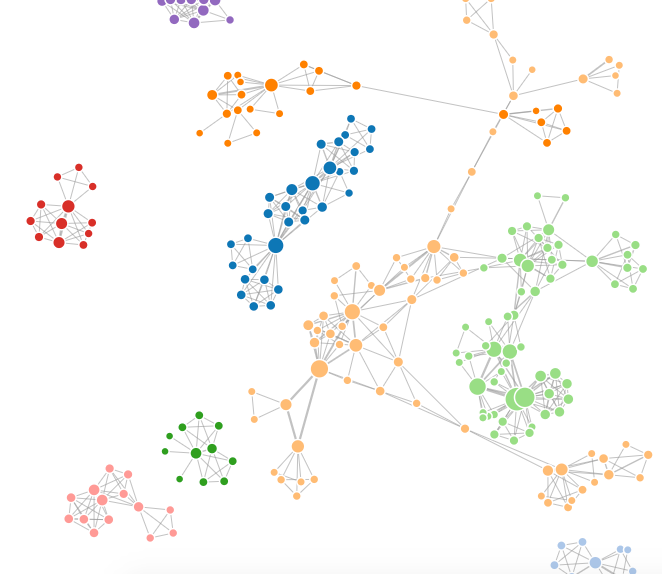
\includegraphics{img/groups_vis.png}
\caption{Coauthorship network of the visualization methods papers
surveyed in \autocite{vehlow_state_2015}. Nodes represent authors, with
weighted links indicating co-authorship. Nodes in this view are colored
by the top level of the hierarchical Infomap community assignment, and
roughly correspond to labs and institutions. Available at
\url{http://students.washington.edu/jporteno/groups/}}\label{fig:groupsvis}
\end{figure}

I represent the co-authorship network using D3
\autocite{bostock_d3:_2011} as a node-link diagram, which is a very
common way of visualizing networks. The nodes are visualized using a
force-directed algorithm, in which forces of attraction and repulsion
are applied to nodes and links and then placed so as to minimize the
energy. Interestingly, the force-directed layout has been shown to be
equivalent to the commonly used modularity quality function for
communities \autocite{noack_modularity_2009}---this is why a
visualization of a network that uses this layout can show implicit
community structure by grouping similar nodes together visually.

\subsection{Labs involved in visualizing group structure in
networks}\label{labs-involved-in-visualizing-group-structure-in-networks}

Using this system can help to identify some of the key researchers in
this area and the relationships between them. To find the labs, I can
search the web for their lab or university websites. By doing this, I
was able to find a number of labs doing interesting work.

One community that pops out appears in the middle of the largest
connected component, with several large and well-connected nodes.
Perhaps unsurprisingly, this community represents the authors of the
survey paper (and the curators of the bibliography data behind the
visualization). This is the University of Stuttgart Visualisation
Research Centre (VISUS), and includes Daniel Weiskopf, Fabien Beck and
others. It also used to include then-PhD student and lead author of the
survey paper Corinna Vehlow. An interesting recent paper from this lab
is \autocite{vehlow_visualizing_2015}, in which dynamically evolving
community structure is visualized as rectangular blocks (in a way
resembling the alluvial diagrams in Rosvall and Bergstrom
\autocite{rosvall_mapping_2010} see Fig.~\ref{fig:alluvial}), and these
are combined with node-link representations of the community subgraphs.
Fig.~\ref{fig:vehlow} shows the evolution of a network of soccer teams
over time.

\begin{figure}
\centering
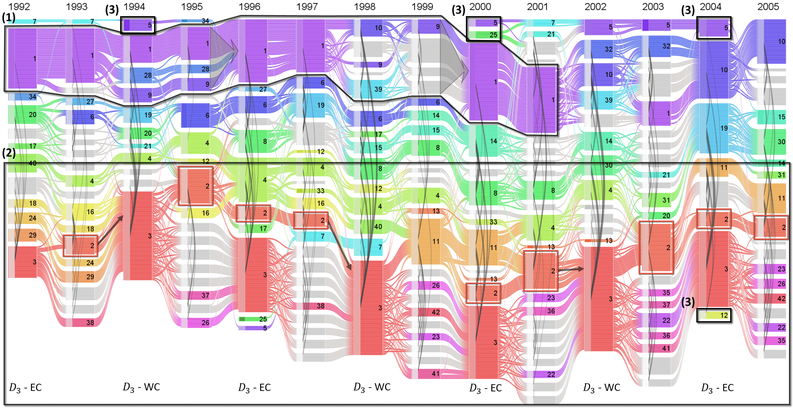
\includegraphics{img/vehlow2015_fig7_dynamic.png}
\caption{Evolution of the community structure of a network of soccer
matches from 1992 to 2005 (teams are connected if they played each
other) From Vehlow et
al.~\autocite{vehlow_visualizing_2015}.}\label{fig:vehlow}
\end{figure}

Close to the Stuttgart lab is the team at LaBRI at the University of
Bordeaux, France. Researchers here include Romain Bourqui and David
Auber. Dr.~Auber appears to work closely with researchers at the
University of British Columbia including Tamara Munzner and Daniel
Archambault. An interesting paper from the LaBRI group is
\autocite{sansen_adjasankey:_2015}, where one technique they use to show
hierarchical structure involves assigning similar color to similar
nested groups.

Other groups can be seen in the largest connected component. A group of
researchers appears as a maroon community; this is the MArVL group at
Monash University in Melbourne, Australia, which includes Kim Marriott
and Tim Dwyer (I have seen Dr.~Dwyer's work before---he created cola.js,
a constraint-based graph visualization layout that works with D3). The
UC Davis Center for Visualization appears as a mostly blue community.
The University of Arizona Graph and Map Algorithm (GAMA) Lab, headed by
Stephen Kobourov, is well connected in the component. An interesting
paper out of this last lab is \autocite{gansner_gmap:_2010}, in which
communities are visualized to look like cartographic maps. This method,
which the authors call GMap has a pleasing aesthetic that people might
find preferable to the standard node-link diagram, as many people are
turned off by the ``hairball'' that tends to result from the standard
approach. Indeed, the authors use their mapping technique to visualize a
co-authorship network (Fig.~\ref{fig:gmap}), and this may be a superior
way to visualize this data than what I have done. Another paper
\autocite{saket_map-based_2015} found that the cartographic map
technique improved people's recall of data.

\begin{figure}
\centering
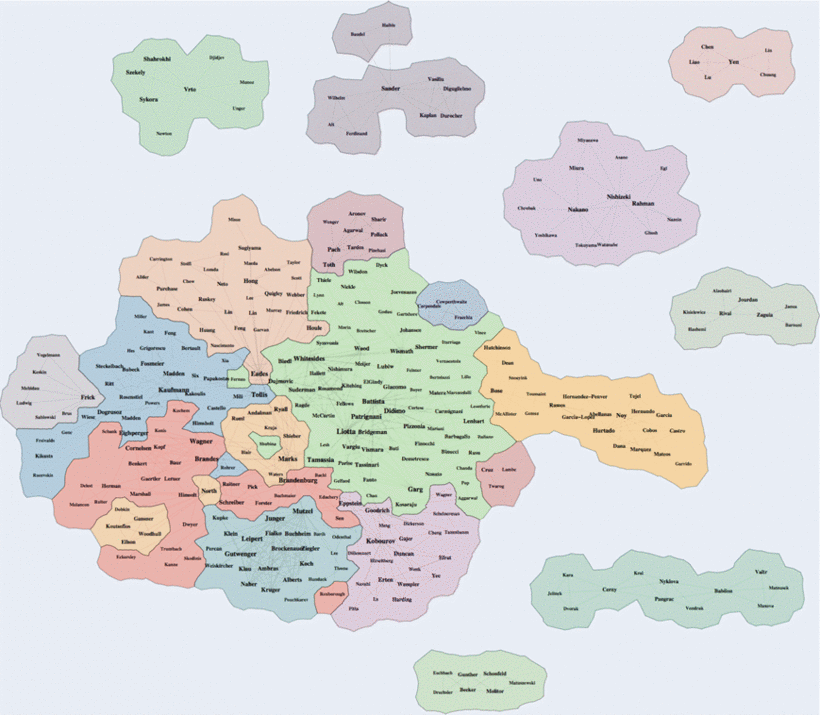
\includegraphics{img/ganser2010_fig6_gmap.png}
\caption{GMap \autocite{gansner_gmap:_2010} representation of an author
collaboration network among visualization ressearchers.}\label{fig:gmap}
\end{figure}

Some labs are represented in the smaller components as well. One such
component contains two labs in China---the Tong Ji Intelligent Big Data
Visualization Lab, headed by Nan Cao; and the VisLab at Hong Kong
University, headed by Huamin Qu. One paper from the VisLab is
\autocite{wu_interactive_2015}, in which contour overlays using Voronoi
cells are superimposed over nodes to show communities.

\subsection{Visualizing group structure in graphs: State of the art and
open
problems}\label{visualizing-group-structure-in-graphs-state-of-the-art-and-open-problems}

The review article (\autocite{vehlow_state_2015}) proposes a taxonomy of
methods for visualizing group structure in graphs. This taxonomy
characterizes techniques along two axes. The group structure taxonomy
identifies the type of groups being visualized---disjoint flat groups,
overlapping flat groups, disjoint hierarchical groups, or overlapping
hierarchical groups. The group visualization taxonomy characterizes the
way that the group structure is presented in the visualization---node
attributes (such as color), juxtaposed views, superimposed views, or
embedded views. The authors organize all of the papers in their review
according to this taxonomy and include this information in their curated
bibliography. This taxonomy is useful for navigating the space of
visualizing communities, and can help find examples of techniques that
have been used.

Vehlow et al. also include a discussion of open research challenges in
visualizing group structure in graphs, informed by interviews with
experts in the field. They identify five main areas with work to do:

\begin{enumerate}
\def\labelenumi{\arabic{enumi}.}
\tightlist
\item
  Representating \emph{time-varying} group structure, especially the
  simultaneous representation of group evolution and graph topology.
  Similarly, we need ways of \emph{comparing} sets of graphs.
\item
  More \emph{data complexity}---for instance, visualizing fuzzy
  overlapping groups, in which any node can be assigned to multiple
  communities, possibly with different probabilities.
\item
  \emph{Scalable approaches}---for example, representing community
  assignment by coloring the nodes becomes difficult for more than seven
  groups.
\item
  \emph{Interactive visualizations} provide many possibilities, and
  there already exist many examples, but much of this space remains to
  be explored.
\item
  The question of how to best \emph{evaluate} visualization techniques
  is still open, including the identification of \emph{tasks} that these
  visualizations can support.
\end{enumerate}
